\documentclass[sigplan,review]{acmart}

\usepackage{microtype}

%%
%% \BibTeX command to typeset BibTeX logo in the docs
\AtBeginDocument{%
  \providecommand\BibTeX{{%
    Bib\TeX}}}

%% Rights management information.  This information is sent to you
%% when you complete the rights form.  These commands have SAMPLE
%% values in them; it is your responsibility as an author to replace
%% the commands and values with those provided to you when you
%% complete the rights form.
%%% The following is specific to FUNARCH '25 and the paper
%%% 'Six Years of FUNAR: Functional Training for Software Architects'
%%% by Michael Sperber.
%%%
\setcopyright{acmlicensed}
\acmYear{2026}
\copyrightyear{2026}
\acmConference[FUNARCH '26]{Proceedings of the 4th ACM SIGPLAN
  International Workshop on Functional Software Architecture}{August
  29, 2026}{Indianapolis, USA}
\acmBooktitle{Proceedings of the 4th ACM SIGPLAN International
  Workshop on Functional Software Architecture (FUNARCH '26), August
  29, 2026, Indianapolis, USA}

%%
%% Submission ID.
%% Use this when submitting an article to a sponsored event. You'll
%% receive a unique submission ID from the organizers
%% of the event, and this ID should be used as the parameter to this command.
%%\acmSubmissionID{123-A56-BU3}

%%
%% For managing citations, it is recommended to use bibliography
%% files in BibTeX format.
%%
%% You can then either use BibTeX with the ACM-Reference-Format style,
%% or BibLaTeX with the acmnumeric or acmauthoryear sytles, that include
%% support for advanced citation of software artefact from the
%% biblatex-software package, also separately available on CTAN.
%%
%% Look at the sample-*-biblatex.tex files for templates showcasing
%% the biblatex styles.
%%

%%
%% The majority of ACM publications use numbered citations and
%% references.  The command \citestyle{authoryear} switches to the
%% "author year" style.
%%
%% If you are preparing content for an event
%% sponsored by ACM SIGGRAPH, you must use the "author year" style of
%% citations and references.
%% Uncommenting
%% the next command will enable that style.
%%\citestyle{acmauthoryear}


%%
%% end of the preamble, start of the body of the document source.
\begin{document}

%%
%% The "title" command has an optional parameter,
%% allowing the author to define a "short title" to be used in page headers.
\title{Local-First Distributed Configuration}
\subtitle{Experience Report}

%%
%% The "author" command and its associated commands are used to define
%% the authors and their affiliations.
%% Of note is the shared affiliation of the first two authors, and the
%% "authornote" and "authornotemark" commands
%% used to denote shared contribution to the research.
\author{Michael Sperber}
\email{sperber@deinprogramm.de}
\affiliation{%
  \institution{Active Group GmbH}
  \streetaddress{Hechinger Straße 12/1}
  \city{Tübingen}
  \country{Germany}
  \postcode{72072}
}

%%
%% The abstract is a short summary of the work to be presented in the
%% article.
\begin{abstract}
  We have been developing a distributed application called
  \textit{Lokalisierung} using functional programming in 2015.
  Lokalisierung configures automatically mobiles devices in an a large
  organization of auto-inspection shops. It uses peer-to-peer
  synchronization to distribute configuration data among the devices,
  without the use of a central server.  This paper describes the
  original design and evolution of the system.  Specifically, we
  highlight how the event-based architecture supports synchronization
  but also enables flexibility for changes after the original rollout
  such as undoing configuration changes, and database thin out.  We
  also reflect on some design and implementation mistakes during its
  10-year history.
\end{abstract}

%%
%% The code below is generated by the tool at http://dl.acm.org/ccs.cfm.
%% Please copy and paste the code instead of the example below.
%%
\begin{CCSXML}
<ccs2012>
   <concept>
       <concept_id>10010520.10010521</concept_id>
       <concept_desc>Computer systems organization~Architectures</concept_desc>
       <concept_significance>500</concept_significance>
       </concept>
   <concept>
       <concept_id>10011007.10010940.10010971.10010972</concept_id>
       <concept_desc>Software and its engineering~Software architectures</concept_desc>
       <concept_significance>500</concept_significance>
       </concept>
   <concept>
       <concept_id>10011007.10011006.10011008.10011009.10011012</concept_id>
       <concept_desc>Software and its engineering~Functional languages</concept_desc>
       <concept_significance>500</concept_significance>
       </concept>
 </ccs2012>
\end{CCSXML}

\ccsdesc[500]{Computer systems organization~Architectures}
\ccsdesc[500]{Software and its engineering~Software architectures}
\ccsdesc[500]{Software and its engineering~Functional languages}

%%
%% Keywords. The author(s) should pick words that accurately describe
%% the work being presented. Separate the keywords with commas.
\keywords{functional programming, software architecture, education}
%% A "teaser" image appears between the author and affiliation
%% information and the body of the document, and typically spans the
%% page.
\received{1 June 2026}

%%
%% This command processes the author and affiliation and title
%% information and builds the first part of the formatted document.
\maketitle

\section{Introduction}

In 2015, we (that is, Active Group, a small software consultancy in
Germany that uses functional programming for all of our projects) were
tasked with implementing an application for a large
auto-inspection-shop organization for configuring its new fleet of
over 1000 mobile devices.

Each auto-inspection shop has multiple lanes, each of which can take
in a car.  At the end of each lane sits a desk closet with a printer
and various pieces of inspection equipment.  Previously, the closed
had also contained a desktop PC permanently hooked up to this
equipment.  The organization had decided to replace the closed-bound
PCs by mobile devices (called \textit{MEG}s), each assigned to an
employee rather than a place. Employees move around frequently, both
between the lanes of a single shop and also between shops.

Each time a MEG operates in a different lane, it needs to connect to
the equipment at that lane. The equipment is accessible
wirelessly. However, various pieces of software inspection needed
reconfiguring. Previously, this had been a laborious manual process
that involved typing in MAC addresses, opening the printer
configuration dialog etc.

Lokalisierung was commissioned to address this problem, to reconfigure
the MEGs as they moved within and between shops.  To that end, each
MEG needs to know the configuration of each place, which also changes
as new shops get launched and equipment gets replaced.  The
organization lacked the infrastructure to operate a central server.
Getting the data live from such a server would have been unrealistic
anyway---auto-shop WiFi is not the most reliable, and the
organization's network did not have enough capacity to support
Lokalisierung. This constraint led all the organization's other
software suppliers to drop out of the project.

We designed an \textit{append-only} data layer that stores
\textit{facts}, as opposed to traditional state-based databases. This
enabled us to tackle the project, resulting in a successful
implementation, launch and now decade-long operation.

% identify locality by IP/mac address

% FIXME: projections
% FIXME: data-model

\paragraph{Overview}  FIXME

\section{Add-Only Database}
\label{sec:addonlydb}

The lack of a central server and the limited availability of network
bandwidth means that each MEG needs to store and access configuration
data locally. Moreover, the MEGs need to synchronize amongst each
other.  This exposes Lokalisierung to the \textit{CAP
  theorem}~\cite{CAP} on distributed databases, which puts limits on
the implementation of distributed databases, specifically those that
store mutable state.

Here is the problem: A lane is configured to be associated with
printer $A$, which breaks.  A user changes the configuration to point
to printer $B$ on MEG $M_1$.  MEG $M_2$, still configured to printer
$A$. It might synchronize with $M_1$, but should it just replace
printer $A$ by $B$ in its printer database?  How does it know which
printer is the correct one?  There might be timestamps associated with
the two different printer configurations, and we might pick the newest
one. However, this requires synchronized clocks and the absence.
Also, as we would find out, changes would often happen in close
temporal proximity. Just storing the seemingly ``current
configuration'' would lead to confusing and difficult-to-trace
situations where somebody's configuration would be overriden without
explanation.

Consequently, instead of a conventional state-based database for the
configuration data, we chose an approach based on storing
\textit{facts}.  While state changes, a fact is something that remains
true and is thus immutable. To illustrate the difference, ``lane 2 has
the FooJet printer with IP 5.5.5.5'' is state, whereas ``Mike said on
May 21, 13:44 that lane 2 has the FooJet printer with IP 5.5.5.5'' is
a fact.  Thus, the database is an evergrowing pool of facts, from
which the current state is derived.  This corresponds to the notion of
\textit{event sourcing}~\cite{FowlerEventSourcing2005,Stopford2018}, as our facts effectively
document events.  (The term ``event sourcing'' was not known to us at
the time.)

The pool of facts may have several facts pertaining to a single
configuration setting<. We use causal order to disambiguate: If a fact
$F_2$ is created that affects the same setting as a fact $F_1$
\emph{that is in the local database when $F_2$ is created}, we note
that $F_2$ \textit{obsoletes} $F_1$.

While there are specialized databases for events, we chose to use
SQLite for storing the facts~\cite{SQLite}.  SQLite requires no
complicated client-server setup and has extensive tool support.  Here
is the initial database schema, with table \texttt{kv} for storing the
facts themselves, and table \texttt{hashes} for storing the obsoletion relationship:
%
\begin{verbatim}
CREATE TABLE kv (
  hash      BLOB   PRIMARY KEY NOT NULL UNIQUE,
  guid      BLOB   NOT NULL,
  property  STRING NOT NULL,
  value     BLOB   NOT NULL,
  meta      STRING NOT NULL);

CREATE TABLE hashes (
  key_hash BLOB NOT NULL,
  obsoleted_hash BLOB NOT NULL,
  FOREIGN KEY(key_hash) REFERENCES kv(hash));
\end{verbatim}
%
The \texttt{guid} field is a unique UID that identifies the subject of
a configuration setting, typically a specific auto shop or lane.  The
\texttt{property} identifies a particular setting, such as
\texttt{printerconfiguration} or \texttt{cdcconfiguration}, the latter
for configuring a particular piece of hardware.  Each fact comes with
metadata in JSON format noting user, machine, and time:
%
\begin{verbatim}
{"user":"mike","machine":"TOURVEL",
 "datetime":"2016-05-04T12:18:47.6872020+00:00"}
\end{verbatim}
%
The \texttt{hashes} table relates ``newer'' facts to the ones they
obsolete. A view combines both tables into a cleaned-up table of
current facts:
%
\begin{verbatim}
CREATE VIEW kvCurrent AS
SELECT hash,guid,property,value,meta
FROM kv
WHERE kv.hash NOT IN
  (SELECT obsoleted_hash FROM hashes)
\end{verbatim}
%
With this schema in place, we built a database-access layer in the
code itself, written in F\#.  While it would have been possible to
just use a SQLite database library directly from the application
code, this has several architectural drawbacks:
%
\begin{itemize}
\item Application code would contain SQL code directly, coupling it to
  the database schema, and making the latter difficult to change.
\item A direct reference to a SQLite library would couple the
  application code to SQLite, making the latter difficult to
  replace. 
\end{itemize}
%
While .NET's ADO.NET database-agnostic framework could have loosened
this coupling, it still would have required \emph{some}
ADO.NET-supported database. We decided early on that we wanted to be
able to use the database access layer without SQLite, using simple F\#
collections, particularly for testing.  (This would become more relevant
later in the project, see Section~\ref{sec:time-machine}.)

Thus, we needed a mechanism for \textit{depencency
  injection}~\cite{FowlerEventDependencyInjection2004}, and
used a free-monad approach~\cite{Swierstra2008} with a data type for
database operations:
%
\begin{verbatim}
type 'a Op =
  | Return of 'a
  | Get of GuidT * PropertyT * (ValueT [] -> 'a Op)
  | Put of FactT * (HashT -> 'a Op)
  ...
  | Atomically of ('a Op) Op
\end{verbatim}
%
The \texttt{Atomically} operation is for transactions. A set of
convenience functions, a \texttt{bind} function, and a builder for
F\# \textit{computation expressions}~\cite{PetricekSyme2014}:
%
\begin{verbatim}
let ret a = Return a
let get guid prop = Get (guid, prop, ret)
let put fact = Put(fact, ignoreAndReturn ())
...
let atomically (op: 'a Op): 'a Op =
  Atomically (bind op (fun v -> Return (Return v)))

let rec bind<'b, 'a> (opB: 'b Op) (f: 'b -> 'a Op)
      : ('a Op) =
    match opB with
    | Return b -> f b
    | Get (g, p, cont) ->
      Get (g, p, (fun v -> bind (cont v) f))
    | Put (d, cont) ->
      Put (d, (fun v -> bind (cont v) f))
    | Atomically op ->
      Atomically (bind op (fun op' ->
                           Return (bind op' f)))

type DbBuilder() =
    member _this.Return(v) = Return v
    member _this.ReturnFrom(m) = m
    member _this.Bind(m,f) = bind m f
let db = DbBuilder()
\end{verbatim}
%
Computation expressions allow writing the application code in a
straightforward, sequential way, while clearly limiting database
access code to functions with \texttt{Op} return type. The codebase
includes two different interpreters for \texttt{Op} values, one
accessing SQLite, one using in-memory F\# collections.

\section{Synchronization}

\begin{figure}[tb]
  \centering
  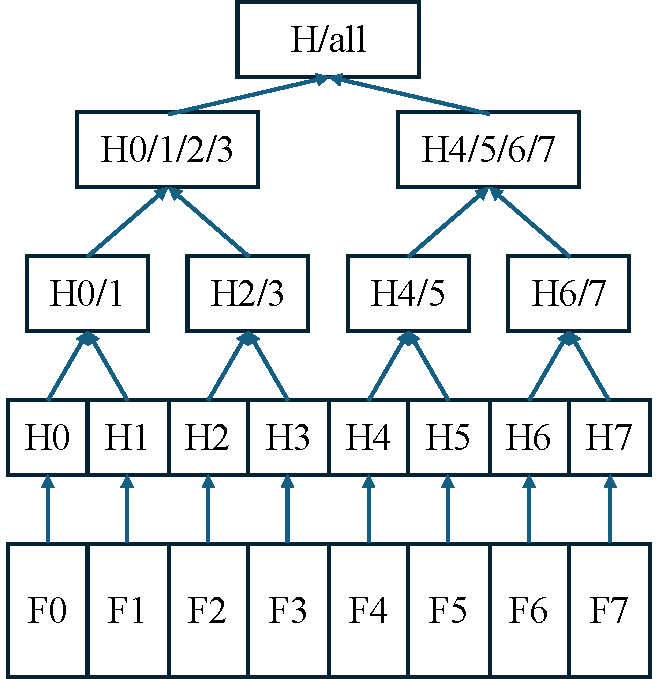
\includegraphics[width=0.8\columnwidth]{merkle-tree}
  \caption{Merkle tree}
  \label{fig:merkle-tree}
\end{figure}

With the facts database and obsoletion relation in place, it becomes
feasible to synchronize the facts between two MEGs efficiently. The
standard method for this is a \textit{Merkle tree}:

A Merkle tree sits atop the set of facts, each of which has a
hash---see Figure~\ref{fig:merkle-tree}. The individual hashes $H_i$
of facts $F_i$ form the leaves of the tree. Going up the tree, each
node points to a number of nodes below, and is labelled with a hash
that is the result of combining the hashes from the level
below. This means that the hash that labels each node summarizes the
facts below.  The top hash summarizes the entire set of facts.

The synchronization algorithm implicitly constructs the Merkle tree
for both MEGs involved, using the bits of the fact hashes as paths
down the tree.  The algorithm traverses the tree top-down, sending
hashes to the other side, and keeping a set of candidate hashes whose
facts might need transmitting to the other side.

If the top hashes agree, both sets of facts are the same, and no
synchronization is necessary. Otherwise, both sides need to descend a
level, and send its hashes to the other side as potential
candidates. Those hashes that agree can be removed from the
candidates, and the algorithm descends to the next level only from these
candidates. When it finally reaches the lowest level, the remaining
candidates identify those hashes that need to be transmitted to the
other side.

Each MEG determines when to invoke the algorithm by sending UDP
broadcasts containing the top hash into the local network on a number
of occasions:
%
\begin{itemize}
\item when the MEG enters a network (typically when the car containing
  it drives onto the parking lot of the shop),
\item when the network configuration changes,
\item when new facts were added.
\end{itemize}
%
When an MEG receives such a UDP broadcast, it compares the broadcast's
top hash with its own, and, if they differ, engages in a
synchronization with the other side. This tactic has proved
exceedingly effective in keeping all MEGs sufficiently updated to be
usable wherever they go.

The synchronization algorithm is organized into three components:
%
\begin{description}
\item[Algorithm] This implements the synchronization algorithm as a
  pure function.
\item[Protocol] This implements serialization of the messages
  required by the algorithm.
\item[Communication] This orchestrates the two to implement
  synchronization between MEGs.
\end{description}
%
The only dependency between Protocol and Algorithm is the common
message datatype, making both independently testable:
%
\begin{verbatim}
type Msg =
| IHaveFingerprints of MerkleFingerprintSet
| HereAreBlockHashes of list<Hash.T>
\end{verbatim}
%
The \texttt{IHaveFingerprints} message tells the other side for each
successive level the \textit{fingerprints} of the candidates.  A
fingerprint is just a combination of the hash of the corresponding
node along with the path leading to that node from the root.  When the
algorithm reaches the lowest level, it generates a
\texttt{HereAreBlockHashes} message containing the blocks to be
transmitted to the other side.

The signature of the algorithm function is as follows:
\begin{verbatim}
let synchronizationRound (allHashes: Set<Hash.T>)
                         (treeSet: MerkleTreeSet)
                         (msg: Msg)
 : Choice<Msg * MerkleTreeSet, list<Hash.T>> = ...
\end{verbatim}
%
The function takes as argument the set of candidate subtrees and the
message that just came from the other side, and returns either a
message to transmit to the other side along with a set of candidates
for the next round, or the blocks received from the other side.

The implementation of \texttt{synchronizationRound} is fairly
involved, and many mistakes were made implementing it. However, the
correctness of synchronization is easy to write as a QuickCheck
property~\cite{QuickCheck2000} shown in
Figure~\ref{fig:sync-quickcheck}.  The \texttt{checkSynchronizeWorked}
function takes four sets of blocks, \texttt{blocks1} and
\texttt{blocks1'} being the blocks present and received on one side,
and \texttt{blocks2} and \texttt{blocks2'} on the other side.  This
was the main test for validating the implementation before its
original deployment in 2015, and no bugs have been detected since.

\begin{figure*}[tb]
  \centering
\begin{verbatim}
let checkSynchronizeWorked (blocks1: list<Block<'A>>) (blocks2: list<Block<'A>>)
                           (blocks1': list<Block<'A>>) (blocks2': list<Block<'A>>) =
  let hashes1 = List.map blockHash blocks1 |> Set.ofList
  let hashes2 = List.map blockHash blocks2 |> Set.ofList
  let hashes1' = List.map blockHash blocks1' |> Set.ofList
  let hashes2' = List.map blockHash blocks2' |> Set.ofList
  let allHashes = Set.union hashes1 hashes2
  Set.union hashes1 hashes1' |> should equal allHashes
  Set.union hashes2 hashes2' |> should equal allHashes
  Set.isSubset (Set.ofList blocks1') (Set.ofList blocks2) |> should be True
  Set.isSubset (Set.ofList blocks2') (Set.ofList blocks1) |> should be True

[<Test>]
member x.``synchronization works for arbitrary lists of blocks`` () =
    Prop.forAll(Arb.from<Set<Block<byte[]>> * Set<Block<byte[]>>>) (fun (bs1, bs2) ->
        let blocks1 = Set.toList bs1
        let blocks2 = Set.toList bs2
        let (blocks1', blocks2') = synchronize schema1 blocks1 blocks2
        checkSynchronizeWorked blocks1 blocks2 blocks1' blocks2'
    )|> AssertProperty
\end{verbatim}
  \caption{QuickCheck test for synchronization algorithm}
  \label{fig:sync-quickcheck}
\end{figure*}
%
Synchronization is asynchronous to the application itself: The
Communication component needs to call back into the application to
retrieve available blocks and store blocks received in a
synchronization run.  To that end, application supplies a
\textit{synchronization context} of the following type:

\begin{verbatim}
type SyncContext<'A> when 'A : equality = {
  ahash: 'A -> Hash.T
  serializer: Serializer<'A>
  getHashes: unit -> Async<list<Hash.T>>
  getBlocks: list<Hash.T> -> Async<list<Block<'A>>>
  saveBlocks: list<Block<'A>> -> Async<unit>
}
\end{verbatim}
%
This context abstracts over the type of the blocks \verb|'A|, even
though this type is fixed in the application.  While this is generally
good decoupling practice, it enabled development of the
synchronization algorithm independently of the rest of the
application, before the type of the blocks was even known.  More
importantly, it simplified unit testing of the Communication
component, where small, synthetic data blocks can be used rather than
the structured values required by the Lokalisierung application.

\section{Conflict Resolution}
\label{sec:conflicts}

If two users create different settings on their MEGs and these two
MEGs synchronize, it is unclear to Lokalisierung which setting to use.
Internally, Lokalisierung represents such settings as follows:
%
\begin{verbatim}
type Val<'a> when 'a : comparison =
| Absent
| Good of 'a
| Conflict of Set<WithMeta<'a>>
\end{verbatim}
%
During initial development, we assumed users would change settings
mostly when in physical proximity to the lanes affected, and
immediately propate them throughout the auto shop, making such
conflicts rare.

Therefore, we assumed such conflics could be resolved on the spot.  We
made Lokalisierung detect conflicts after synchronization and display
a dialog requiring users to resolve it.  (The \texttt{WithMeta} type
contains the metadata from the append-only database, allowing the
dialog to display information about who made a conflicting setting,
when and and where.)

This strategy seemed obvious to us at the time, but proved completely
unworkable in practice, as our assumption about the frequency and
nature of conflicts proved false.  From the users' perspective,
Lokalisierung would pop up a dialog unpredictably.  Worse, it would
appear on both MEGs involved in the synchronization, with no clear
responsibility as to who should do what. We had not properly accounted
for the fact that we had created a distributed system.

Our knee-jerk reaction was to automate filling out the dialog.  This
proved disastrous, as it would happen on both MEGs involved in the
synchronization, creating two distinct resolution facts. These would be
exchanged on the next synchronization, creating another conflicts, and
so on, creating an avalanche of facts.  Fortunately, this was detected
within a few minutes of deployment and stopped.  The lesson here was
to now create synthetic facts ever.

We ultimately settled on the following conflict strategy:
%
\begin{itemize}
\item If there are multiple facts for the same setting, Lokalisierung
  compares the values: If they are the same, it assumes that to be the
  correct setting. This eliminated most conflicts.
\item When the values are different, the UI displays the relevant
  settings in red, but does not pop up disruptive dialogs. The user
  can then make a new setting, resulting in a fact obsoleting the
  conflicting facts.
\end{itemize}
%
This strategy proved acceptable to the users, even though we were
never able develop a good mental model of the usage
patterns.

\section{Data Modeling and Time Machine}
\label{sec:time-machine}

Initial versions of Lokalisierung would retrieve settings individually
from the append-only database, effect the corresponding configuration
changes directly and transfer them to corresponding fields in the
UI. The resulting coupling of the database structure to the UI
structure, while an architectural problem in many applications, never
proved problematic in Lokalisierung, mainly as the configuration
structure has remained largely the same.

However, after Lokalisierung had been in use for a while, shop
managers informed us that they often wanted to roll back erroneous
settings.  (Again, we never determined the usage pattern that would
lead to this problem.)  Fortunately, the append-only database
contained the entire history of configuration changes, so all old
settings were still present.  Consequently, we set out to build a
\textit{time machine} that would allow users to go back to any past
setting state for a given shop.

Note that this is not simply a matter of removing newer facts from the
database: The nature of the append-only database does not allow it.
Moreover, we wanted to preserve an audit log of changes and rollbacks.
Thus, Lokalisierung needs to make changes on top of whatever the
current configuration is to re-create a past state.  Then we could
compare it to current state, and re-play the differences on top of the
current state.

In order to re-create the past state, we needed a view on a subset of
the facts. We did this by selecting the facts of the shop in question
up to a certain point in time, and using that to populate the
in-memory implementation of the append-only database.  (Which we had
originally created only for testing purposes.)  This required no
changes to the codebase, and the dependency mechanism we had
originally created for testing purposes paid off here as well.

In order to coherently represent and display the changes that would be
made, we first created an explicit data model for a shop's
configuration, as well as one for the changes to it:
%
\begin{verbatim}
type Locality = {
  guid: PlaceGuid
  displayName: string
  macAddress: Val<option<MacAddress>>
  networkPrinterConfiguration:
    Val<option<PrinterConfiguration>>
  ...
}
type LocalityChangeDescription =
  | SetDisplayName of string
  | SetPlace of (PlaceGuid * PlaceChangeDescription)
  ...
type PlaceChangeDescription =
  | SetDisplayName of string
  | SetRank of int
  ...
\end{verbatim}
%
Note that these datatypes had previously been implicit, and
Lokalisierung had turned configuration changes directly into facts and
added them to database.  Users had to follow up mistakes with more
changes.  Making both the \texttt{Locality} representation and the
changes explicit not only helped us implement the time machine.  It
also allowed us to decouple making the changes from persisting them.
We made the regular configuration-change UI operate on the
\texttt{Locality} datatype, create \texttt{ChangeDescription} values
and display the corresponding changes, and offer an explicit ``Save''
button to persist them.

\section{Database Thinning and Protocol Evolution}

In 2024, the client asked us to do something about the size of the
database, which had grown to several hundred megabytes.  This was not
so much a space problem as it made synchronization slow for new MEGs.
Many of the facts being synchronized had long been obsoleted, and were
not realistic candidates for restoration by the time machine.  Thus,
our client commissioned us to reduce the size of the database by
deleting such irrelevant facts---\textit{thinning}.

Deleting facts means deleting them from the \texttt{kv} table
described in Section~\ref{sec:addonlydb}. As this table contained the
\texttt{hash} primary key referenced by the \texttt{hashes} table, a
migration of the database schema was necessary.  This migration
introduces a new table \texttt{all_hashes} containing just the hashes
of all facts, past and present, with the new \texttt{kv} and
\texttt{hashes} table referencing it:
%
\begin{verbatim}
CREATE TABLE all_hashes (
  hash BLOB PRIMARY KEY NOT NULL UNIQUE
  );
CREATE TABLE kv (
  ...
  FOREIGN KEY(hash) REFERENCES all_hashes(hash)
  );
CREATE TABLE hashes (
  ...
  FOREIGN KEY(key_hash) REFERENCES all_hashes(hash)
  );
\end{verbatim}
%
With this new schema, Lokalisierung could remove facts from the
database by just deleting them from \texttt{kv}. We settled deleting
facts that had been long obsoleted---before a certain date. The date
of a fact's creating were recorded in the \texttt{meta} field of the
\texttt{kv} table as a field in a JSON object, which SQLite
fortunately can access directly.  Consequently, thinning out can be
done with a single SQL \texttt{DELETE}, making it quite fast:
%
\begin{verbatim}
DELETE FROM kv WHERE kv.hash IN
(SELECT kv_obsoleted.hash
FROM kv as kv_obsoleted, kv as kv_current, hashes
WHERE hashes.obsoleted_hash=kv_obsoleted.hash AND
      hashes.key_hash=kv_current.hash AND
      json_extract(kv_current.meta, '$.datetime')
        < :obsoletedBefore)
\end{verbatim}
%
The \texttt{:obsoletedBefore} placeholder gets bound to cutoff for
the date of obsoletion.

\section{Missteps}
This section documents some architecturally relevant missteps that
happened during development.

\paragraph{Unstable hashes} 
FIXME always constrain the database

\paragraph{Incorrect projections} FIXME

\paragraph{Protocol fail} FIXME serialization library, deserializing
protocol version

\paragraph{Untestable configuration manager} FIXME

\paragraph{Unnecessary projections} FIXME


\paragraph{Overly abstract data modeling}

\section{Lessons learned}

events good 
explicit data modeling good

database constraints if possible



\begin{acks}
  I thank Andreas Bernauer for the early design of the add-only
  database, and Helmut Dobretzberger for maintaining Lokalisierung
  over the years.
\end{acks}
%%
%% The next two lines define the bibliography style to be used, and
%% the bibliography file.
\bibliographystyle{ACM-Reference-Format}
\bibliography{funarch-lokalisierung}

\end{document}
\endinput
%%
%% End of file `sample-sigplan.tex'.
